\section{Freemium}

Con un prodotto Freemium si propone un servizio base ad una vasta platea di
utenti gratuiti e un servizio avanzato ad una fetta ristretta di utenti a
pagamento.

\begin{example}[Skype]\label{es:bmi:skype}
Skype ad esempio offre un insieme di funzionalità gratuite, come ad esempio le
chiamate web. Di fianco a questo servizio ne viene offerto uno a pagamento
(chiamato Skype-out) che offre chiamate telefoniche per chi vuole chiamare
telefoni ``tradizionali'', e non solo un PC/smartphone tramite la connessione
dati.

\noindent L'utente ha bisogno di comprare dei crediti telefonici e poi ha la
possibilità di chiamare un telefono ordinario.

\noindent Skype ha vinto nella gestione dei costi infrastrutturali:
chi ha inventato Skype era una software house e quindi hanno trovato un modo per inviare i pacchetti voce appoggiandosi sulla infrastruttura degli operatori telefonici classici, evitando i costi dovuti all'infrastruttura. Ciò si ripercuote sugli utenti, permettendo loro di risparmiare sul costo della singola chiamata.
\end{example}

\noindent Tutti i modelli Freemium che funzionano come
nell'Esempio~\ref{es:bmi:skype} hanno delle caratteristiche in comune, come,
prima di tutto, la base di utenti.
Fondamentale risulta essere il \textbf{tasso di conversione} degli utenti, che passano dal modello base a quello a pagamento. Questa è una metrica molto importante.

Un problema di questo modello di business è che nessun utente passi all'account
a pagamento: in questo caso il modello non funziona e si finisce col
fallimento. Anche l'offerta gratis deve risultare appetibile all'utenza finale,
perché le persone devono essere attratte ad usare il prodotto offerto
gratuitamente. Essendo che i costi che un'azienda deve sostenere con questo
modello sono molteplici l'impatto che un utente ``free'' ha sui costi
dell'azienda dev'essere molto basso, altrimenti si incorre nel fallimento.
La \textit{customer relationship} dev'essere la più automatizzata possibile,
perché se gli utenti free ricorrono alla assistenza tecnica l'azienda ci sta
perdendo solamente, senza nessun ricavo.
L'offerta a pagamento deve essere tale da portare l'utente ``free'' a fare il
salto e diventare premium.

\section{Piattaforme sfaccettate}

Una piattaforma sfaccettata nasce dall'unione due distinti, ma interdipendente,
gruppi di clienti. In questo caso è possibile dare valore ad un gruppo solo se anche l'altro è presente.

\begin{example}[Booking.com]
Ad esempio Booking.com offre la possibilità di ricercare alberghi e di farli
prenotare da utenti privati. Essa fa da ponte tra chi offre alberghi e ci ne
sta cercando per alloggiarci
\end{example}

Questa tipologia di soluzione funziona bene finché ci sono tanti utenti che
usano il servizio ma anche tante offerte disponibili. Se vengono a mancare
anche solo una delle due il sistema crolla. La chiave è che le piattaforme
devono attirare e servire tutti i gruppi contemporaneamente per riuscire a
creare valore.

\begin{example}[Pubblicità]
Un altro esempio di piattaforma sfaccettata sono i giornali. Questi vendono direttamente ai lettori il giornali (singole riviste o abbonamenti), ma anche degli spazi per la pubblicità. Questo modello funziona se ci sono abbastanza lettori da far pagare in modo adeguato le pubblicità. Il prezzo della pubblicità dipende poi dalle dimensioni della pubblicità stessa, dalla posizione nel giornale e dal numero di uscite. In ogni caso \emph{le value proposition offerte a lettori e pubblicitari sono diverse}.
\end{example}

\begin{example}[Console videogiochi]
Un esempio ulteriore di business model sfaccettato sono le console: infatti propongono a giocatori e sviluppatori di videogame value proposition totalmente differenti.
\end{example}


È fondamentale con questo modello riuscire a raggiungere la massa critica.

\chapter{Unboundled company}

Le aziende sono composte di tre tipologie diverse di business, in base al loro focus:
\begin{itemize}
\item customer relationship, focalizzate nel trovare clienti e instaurare un rapporto con loro. Un esempio sono le aziende di consulenza che si basano sulla fiducia degli utenti;
\item innovazione del prodotto, basate sulla creazione di nuovi prodotti o servizi. Esempi sono tutte le startup digitali innovative;
\item infrastrutture: per costruire e gestire piattaforme in grado di generare grossi volumi di compiti ripetutivi, come i produttori di automobili.
\end{itemize}
Queste aziende sono diverse per economia, competitività e imperativi culturali.

\begin{figure}[t]
 \centering
 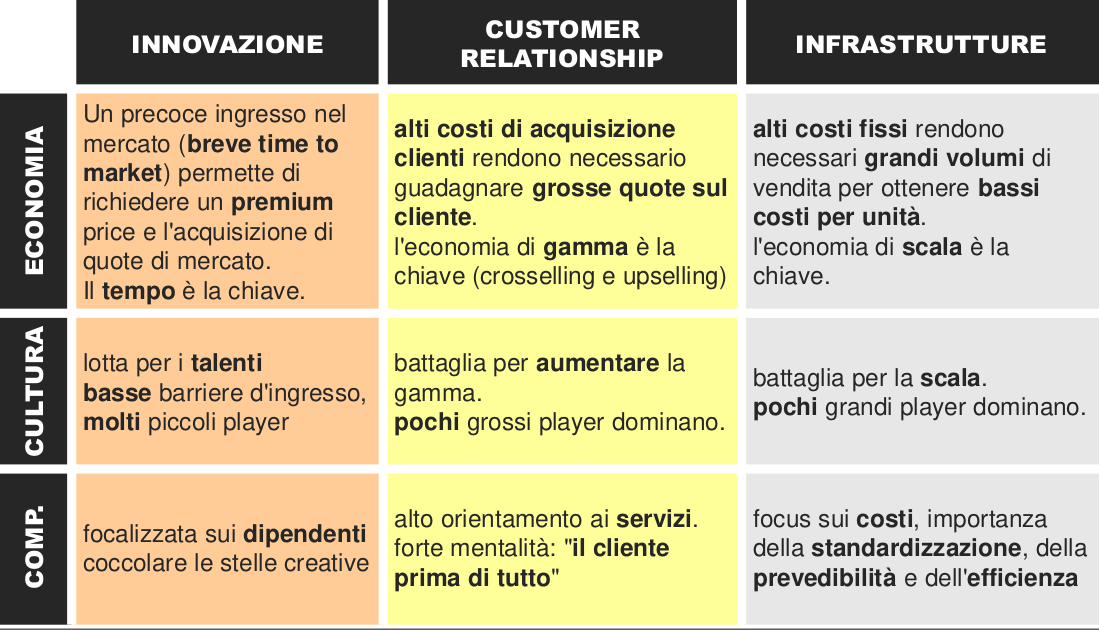
\includegraphics[scale=1.5]{tab_aziende}
 \caption{Tabella caratteristiche del tipo di aziende}
 \label{fig:bmi:tab_aziende}
\end{figure}

\begin{definition}[Time to market]
Il \textit{time to market} di un prodotto è il tempo che passa da quando esso
viene concepito a quando sbarca sul mercato.
\end{definition}

Il time to market varia in base alla tipologia di azienda. Nelle aziende di
innovazione le release sono mensili, dove il loro prodotto cresce. Nell'ambito
industriale di produzione (soprattutto negli elettrodomestici) il time to
market è solitamente di sei mesi, sottolineando come avere un ciclo di release
più breve è fondamentale. Nell'automotive invece, la release di un prodotto
sono lunghi, e si misurano nei blocchi di cinque anni. Adesso nel 2018, Audi,
sta progettando di inserire Chip da inserire nelle auto del 2024. Un campo in
cui le release sono ancora più lunghe sono nel campo farmaceutico: il time to
market è solitamente di 10-15 anni.

Le aziende basate sull'innovazione essendo le uniche che producono quel
prodotto possono chiedere un prezzo premium proprio per la natura stessa di
quello che producono.

\textit{Upselling e crosselling} sono elementi chiave dell'economia nella
customer relationship, questo perché si cerca di massimizzare le vendite sul
singolo utente. Nell'upselling si ha la vendita di differenti diversi prodotti
della stessa tipologia allo stesso cliente, mentre nel crosselling si hanno
diverse tipologie di prodotti.


Fino a poco tempo fa gli operatori di Telefonia Mobile competevano sulla
qualità della loro rete. Al giorno d'oggi questo non vale più molto perché
grazie a vari accordi (e a leggi) è possibile utilizzare la reti di altri
operatori come se questa fosse la mia (Roaming). Come mai? Apparentemente
questo fa perdere l'unicità e la forza del singolo operatore (soprattutto
rispetto alla copertura offerta), ma le aziende telefoniche hanno capito che il
loro key asset non è più la rete, ma il loro brand e la loro relazione con la
base clienti.

Nelle unboundled company vengono scorporate le varie parti di cui l'azienda si
occupa, in modo da migliorare i vari settori.

\begin{figure}[t]
 \centering
 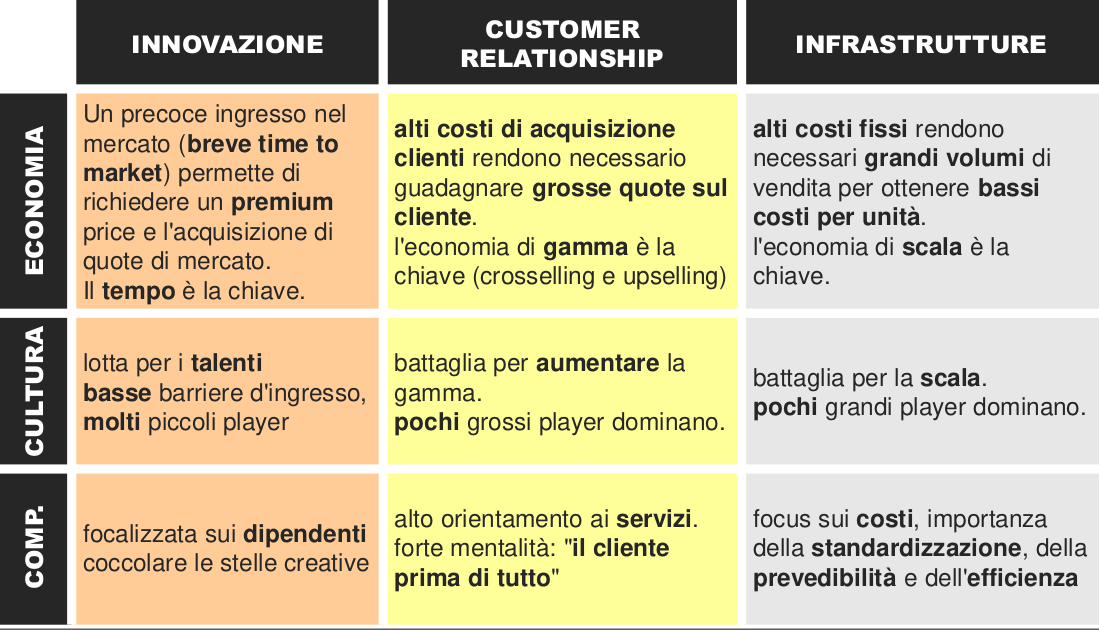
\includegraphics[scale=1.5]{tab_aziende}
 \caption{Esempio unboundled company - Mobile Telco}
 \label{fig:bmi:unboldedcompanytelco}
\end{figure}

\todo{Aggiungere slide 11.32}

\section{Oceano blu}

L'oceano blu si contrappone all'\textbf{oceano rosso}, ovvero un mercato già
saturo e ben stabilito in cui l'unico modo per crescere è rubare le quote di
mercato ai concorrenti. Più il mercato si affolla più difficile diventa
ottenere margini.

\begin{definition}[Oceano blu]
L'\textbf{oceano blu} è uno spazio in cui il mercato è nuovo, in cui la
competizione è nulla o scarsa, in cui la domanda viene creata, non seguita.
\end{definition}

\noindent In questo ``tipo'' di oceano i margini di guadagno e di crescita sono
ampi. La strategia oceano blu è un metodo potente per indagare sulla Value
Proposition e su un business model. Significa aumentare il valore per i clienti
creando nuovi benefici e nuovi servizi e, contemporaneamente ridurre i costi
eliminando caratteristiche e servizi di minor valore.
Da un lato quindi le aziende creano nuovi benefici e servizi andando ad
eliminare le caratteristiche di minor valore.

Può sembrare impossibile, e sicuramente è un'operazione complessa, ma con
metodo e strategie chiare ci si può riuscire e i risultati possono essere
enormi.

\begin{figure}[t]
 \centering
 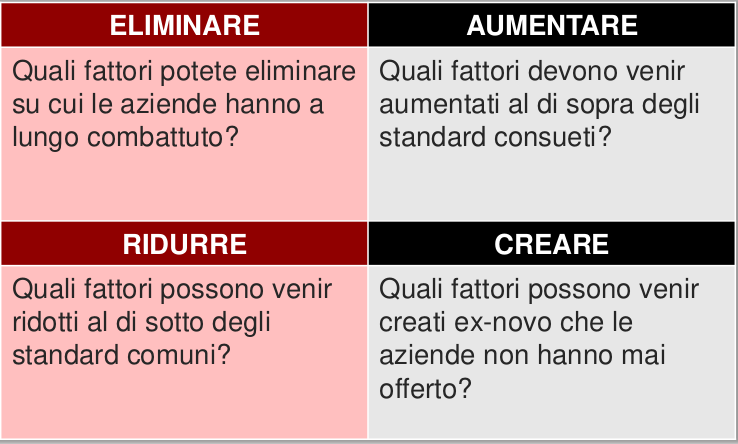
\includegraphics[scale=1.25]{oceano_blu}
 \caption{Caratteristiche dell'oceano blu}
 \label{fig:bmi:oceano_blu}
\end{figure}

Una società per esempio che è riuscito in questo è stato Ryanair, che è
riuscita a portare il concetto di volo, dove la cura del cliente era molto alto
e il prezzo del viaggio era elitario, ad un concetto di volo a prezzo basso.
Sono riusciti in questa opera andando ad analizzare quali erano le ``features''
del prodotto che offrivano che davvero potevano interessare al potenziale
cliente, non mirando più alla persona particolarmente abbiente o al business
man, ma al volo inteso come al mero mezzo di trasporto, per andare dal punto A
a B a prezzi bassi e in tempi ragionevoli. La chiave di volta è stato
domandarsi ``Cos'è che mi genera valore per il mio cliente?''.

Scoprire o creare un oceano blu è un'opera difficilissima, e per niente facile
da realizzare/trovare. È da tenere a mente che inoltre un oceano blu non dura
per sempre.
